%==============================================================================
\section{Combining PINGU with JUNO}
\label{sec:JUNO}
%==============================================================================

\subsection{The JUNO Experiment}
\label{sec:JUNO_exp}

\begin{figure}[thp]
 \centering
 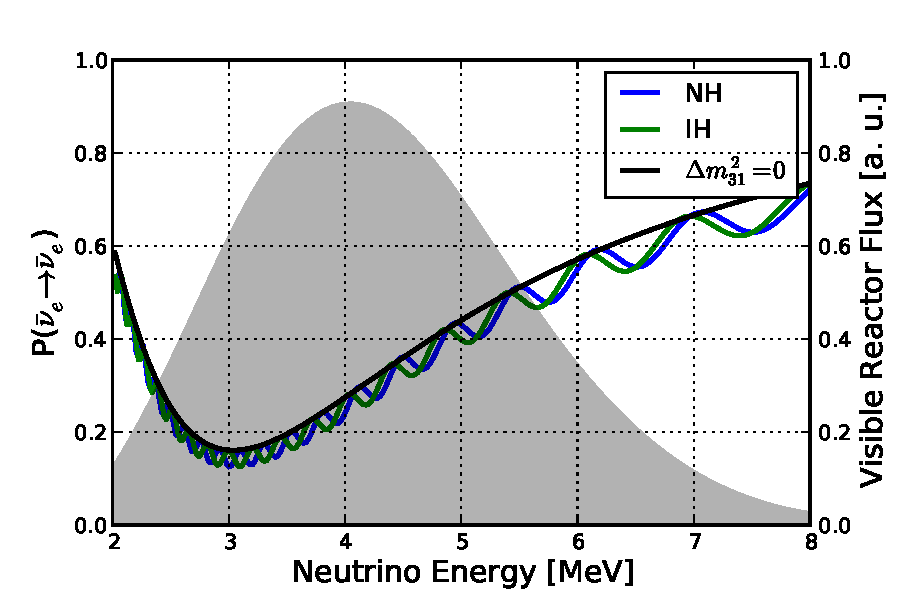
\includegraphics[width=0.7\linewidth]{JUNO_osc_probs}
 \caption{\nuebar survival probability for a baseline of 50\,km, overlaid with
  the un-oscillated nuclear reactor spectrum as it would be detected by JUNO
  (including detector acceptance).}
 \label{fig:JUNO_osc_probs}
\end{figure}

\noindent As already briefly discussed in Sec.~\ref{sec:ReacNuOsc}, 
JUNO\footnote{Short
for Jiangmen Underground Neutrino Observatory.} is a neutrino experiment under
construction in China's Guangdong Province. With its sensitive region at low MeV
energies, it is able to detect supernova and geoneutrinos, yet its main target
are reactor neutrinos from the Taishan and Yangjiang nuclear power plants to be
erected in $\approx 50$\,km distance each. These \nuebar's can be detected via
inverse beta decay:
\begin{equation}
 ^A_Z\mathrm{X} + \nuebar \quad \to\quad  ^A_{Z-1}\mathrm{Y} + e^+
\end{equation}

These \nuebar undergo oscillations that are mostly due to the smaller mass
splitting \dm{21}, but have a fast modulation due to \dm{31}. The vacuum \nuebar
survival probability\footnote{Matter effects can be neglected here.} can be
expressed analytically:
\begin{eqnarray}
 P(\nuebar\to\nuebar)\quad = \quad 1 &-& \cos^4(\thet{13})\,\sin^2(2\thet{12})\,
                            \sin^2\left(\dm{21}\frac{L}{4E}\right) \nonumber\\
                          &-& \cos^2(\thet{12})\, \sin^2(2\thet{13})\,
                            \sin^2\left(\dm{31}\frac{L}{4E}\right) \nonumber\\
                          &-& \sin^2(\thet{12})\, \sin^2(2\thet{13})\,
                            \sin^2\left(\dm{32}\frac{L}{4E}\right)
 \label{eqn:JUNO_osc_probs}
\end{eqnarray}
with $\dm{32} = \dm{31} - \dm{21}$. As shown in Fig.~\ref{fig:JUNO_osc_probs},
for a baseline of $L = 50$\,km this is dominated by the slow \dm{21}
oscillation, corresponding to the first term in (\ref{eqn:JUNO_osc_probs}). On
top of that is a pattern of rapid oscillation originating from the interference
of the second and third term of (\ref{eqn:JUNO_osc_probs}). The exact shape of
this pattern, especially the position of the local minima and maxima, depend on
the mass hierarchy which changes the relative sizes of \dm{31} and
\dm{32}\footnote{Their signs are irrelevant as the outer $\sin^2$ is symmetric
about zero.}.

\begin{figure}[thp]
 \centering
 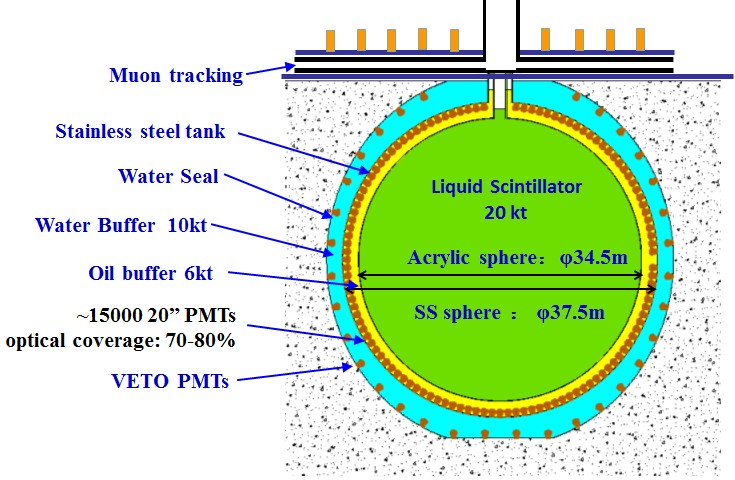
\includegraphics[width=0.7\linewidth]{JUNO}
 \caption{Layout of the JUNO detector. Figure taken from \cite{JUNO2}.}
 \label{fig:JUNO_layout}
\end{figure}

Taking the detector acceptance into account, the expected reactor neutrino
spectrum \cite{JUNO_TDR} is very suitable to observe this signal, as one can see
in Fig.~\ref{fig:JUNO_osc_probs} as well. However, a very precise energy
reconstruction is needed to actually resolve the spectral features associated
with the neutrino mass hierarchy.

With the detector setup shown in Fig.~\ref{fig:JUNO_layout}, a relative
resolution of $3\,\%/\sqrt{E [\mathrm{MeV}]}$ is aimed for. The target volume
is filled with 20\,kt of liquid scintillator to enhance the photon output. This
essentially destroys any directionality of the event signatures, however, no
information about the arrival direction of the neutrinos is needed as the
baseline for the oscillation is known\footnote{In PINGU, the \coszen
information is needed to infer the location where the neutrinos were generated
in the Earth's atmosphere and hence the distance they have travelled.}. The
inner surface of the volume is covered with $\approx 15000$ 20'' PMTs, resulting
in a photocoverage of at least 70\,\%. Tagging and vetoing of atmospheric muons
is ensured by scintillator tiles on top of the detector and a 10\,kt water
Cherenkov detector surrounding the target volume. Natural radioactivity is
buffered in a layer between muon veto and active region filled with 6\,kt of
mineral oil \cite{JUNO2}.

If this precision can indeed be realised, JUNO claims to be able to determine
the neutrino mass hierarchy with a significance of $\approx 3.3\,\sigma$ with a
total $10^5$ recorded neutrino events, corresponding to six years of data taking
\cite{JUNO, JUNO2, JUNO_TDR}. In the following sections a modification of \papa
is described, aiming at a detector simulation for JUNO instead of PINGU in order
to reproduce the reported sensitivity.

\subsection{Simulating JUNO with \papa}
\label{sec:JUNO_sim}

The major difference between the observable signals in PINGU and JUNO is that
PINGU will record a two-dimensional histogram in ($E$,\,\coszen) while in JUNO
only the energy spectrum is measured. Thus only one very narrow zenith bin
with edges at $\coszen = [-0.0039245,\,-0.0039235]$ is simulated, corresponding
to a baseline of 50\,km. In energy, 300 bins between 2\,MeV and 8\,MeV are
used. No oversampling is applied as the oscillation probabilities are
already sufficiently smooth (see Fig.~\ref{fig:JUNO_osc_probs}).

Since only the \nuebar survival probability is relevant for JUNO, which can be
calculated analytically according to (\ref{eqn:JUNO_osc_probs}), the
\texttt{PhysicsSimulation} has been extended by a module doing exactly this
analytical calculation. Avoiding the numerical solution of the Schr\"{o}dinger
equation, the \texttt{PhysicsSimulation} is sped up dramatically.

For the \texttt{DetectorSimulation}, the software itself is not changed,
however the inputs of course have to model the JUNO detector.
The neutrino flux is adopted from \cite{JUNO_TDR} and stored in a table of the
same format as the atmospheric flux tables provided by \cite{HondaSP}. This
flux, shown as an overlay in Fig.~\ref{fig:JUNO_osc_probs}, has the detector
acceptance already folded in, but is only given in arbitrary units. Thus, the
effective area is set to a constant value of 1\,m$^2$ for \nuebar CC and zero
for all other interaction channels while the analysis histograms will be
normalised to $10^5$ \nuebar events before analysis.

The directional reconstruction is parametrised by a single Gaussian with a
fixed width of $10^{-5}$ in \coszen, meaning that all events will stay in
place. As there is only one bin in \coszen, migration of events is impossible
in any case.

The energy reconstruction is represented by a single Gaussian as well, with
mean and width given by
\begin{eqnarray}
 \mu(E) &=& E - 0.8\,\mathrm{MeV} \\
 \sigma(E)/E &=& 4\,\%/\sqrt{E [\mathrm{MeV}] - 0.8} \quad.
\end{eqnarray}
The shift in energy reflects the fact that the visible energy in an inverse beta
decay is smaller than the initial neutrino energy. 511\,keV are needed to
create the $e^+$, which in turn stops to emit Cherenkov light once it falls
below the Cherenkov threshold (\ref{eqn:ChkovThr}), corresponding to a kinetic
energy of $\approx 280$\,keV depending on the optical medium. These two
contributions sum up to $\approx 0.8$\,MeV.
The relative energy resolution refers to the visible energy as well.
Additionally, it has been deteriorated \wrt the published specifications to be
$4\,\%/\sqrt{E_\mathrm{vis} [\mathrm{MeV}]}$. This reflects the fact that the
nuclear power plants used as neutrino sources have several reactor cores that
are up to 500\,m apart from each other. This introduces an uncertainty of 1\,\%
on the baseline $L$, which is equivalent to an additional uncertainty of 1\,\%
in the energy reconstruction as the relevant quantity is $L/E$.

\begin{figure}[thp]
 \centering
 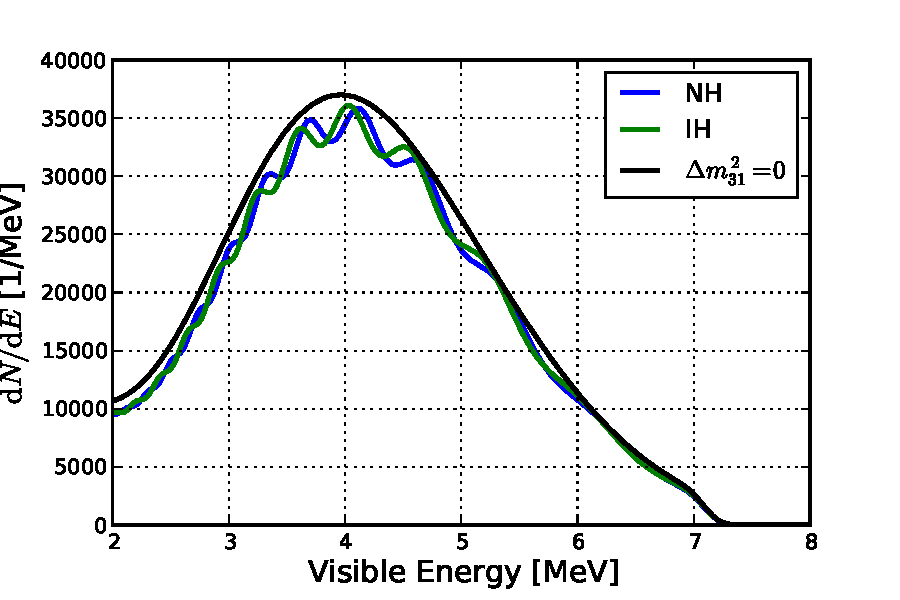
\includegraphics[width=0.7\linewidth]{JUNO_signal}
 \caption{Expected event spectrum in JUNO including all detector effects.}
 \label{fig:JUNO_signal}
\end{figure}

Finally, in JUNO there is no discrimination between cascade-like and track-like 
events as only \nuebar-induced inverse beta decays are expected. Hence, all 
events are classified as cascades and the track channel is not considered for 
the analysis. The resulting observed event distribution for the normal and 
inverted hierarchy case as well as for oscillations with $\dm{31} = 0$ is shown 
in Fig.~\ref{fig:JUNO_signal}.
\enlargethispage{\baselineskip}

\subsection{Preparing the JUNO Signal for Fisher Matrix Analysis}
\label{sec:JUNO_FFT}

\begin{figure}[thp]
 \centering
 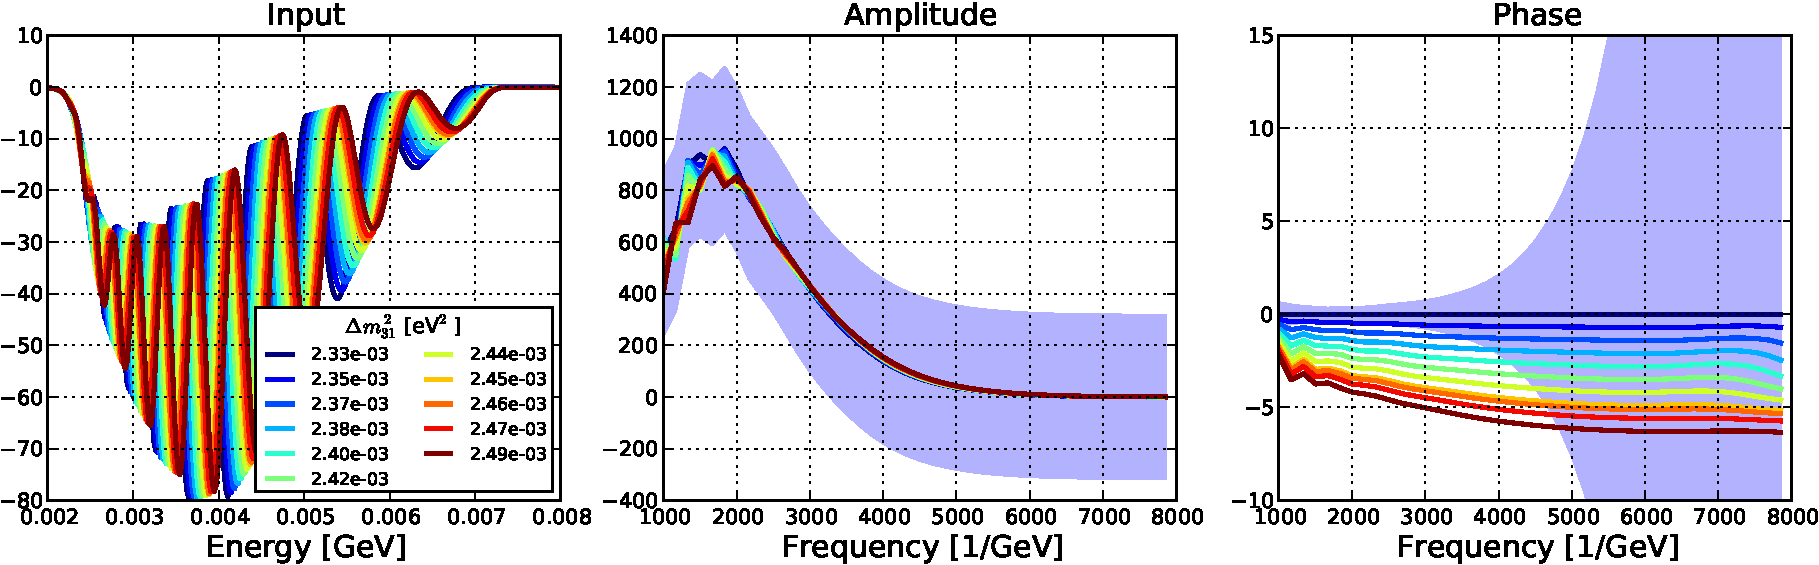
\includegraphics[width=\linewidth]{deltam31_FFT}
 \caption{Linearisation of the detector response to \dm{31} via Fourier 
  transformation. For details, refer to the text.}
 \label{fig:JUNO_FFT}
\end{figure}

\noindent In contrast to PINGU, the analysis histograms for JUNO as shown in 
Fig.~\ref{fig:JUNO_signal} cannot be used for the Fisher matrix analysis 
directly. The reason for this are the rapid oscillations of the event count as 
a function of energy that are the signal to be observed. This means that for a 
given bin in energy, the expected number of events is usually not a linear 
function of the systematic parameters. 
% This is true especially for \dm{31}, as 
% visible in the left panel of Fig.~\ref{fig:JUNO_FFT}. 
% Here, the expected signal 
% for $\dm{31}=0$ (black line in Fig.~\ref{fig:JUNO_signal}) has been subtracted 
% to show the features more clearly.

In order to apply the Fisher matrix formalism, JUNO's response to the 
systematic parameters has to be linearised. As the signal itself is 
oscillatory, the natural choice is to apply a Fourier transformation before 
analysis. To assure an input signal that smoothly fades out to zero at the 
edges of the considered energy interval, the expected signal for $\dm{31}=0$ 
(black line in Fig.~\ref{fig:JUNO_signal}) is subtracted from the actual event 
rates and an exponential cut-off at low energies applied to the result. 

This quantity is shown in the left panel of Fig.~\ref{fig:JUNO_FFT}, the 
non-linearity of the individual bin counts as a function of \dm{31} can clearly 
be seen. It is then fed to the implementation of the fast Fourier transform 
(FFT) algorithm \cite{FFT} provided by the \texttt{numpy} package.

As the input spectrum is real, only positive frequencies have to be considered
in the FFT result. In addition, frequencies below 1/MeV are ignored as they are
subject to large fluctuations. Thus the output of the FFT is a complex
frequency spectrum in the range from 1/MeV to 8/MeV, given as its real and
imaginary part. As the FFT is a linear transform, the error on both is given by
\begin{equation}
 \mathrm{FFT}(\Sigma) = \mathcal{F} \Sigma \mathcal{F}^H \quad,
 \label{eqn:FFTerror}
\end{equation}
where $\mathcal{F}$ is the Fourier matrix, \ie the Fourier transform of the
$n$-dimensional unit matrix where $n$ is the number of bins in the input
series, and $\mathcal{F}^H$ its conjugate transpose. $\Sigma$ is the
covariance matrix of the input data, see \eg \cite{FFT_Error1}.

In this case, the input data are independent bin counts $N_i$ with statistical
errors $\sigma_i = \sqrt{N_i}$, hence $\Sigma$ is diagonal:
\begin{equation}
 \Sigma = \mathrm{diag}(\vec{\sigma})
 = \mathrm{diag}(\sigma^2_1,\,\sigma^2_2,\,\dots,\,\sigma^2_n)
 = \mathrm{diag}(N_1,\,N_2,\,\dots,\,N_n)
\end{equation}
Propagating these properties through (\ref{eqn:FFTerror}) one finds that the
error on both the real and the imaginary part of the FFT output is constant and
proportional to the square root of the total number of bin
entries\footnote{The full error on any observable, \ie entry in the FFT output
spectrum, is given by the square root of the corresponding diagonal element of
the covariance matrix, cf.\ (\ref{eqn:sigma_full}).}:
\begin{equation}
 \Re[\mathrm{FFT}(\Sigma)] = \Im[\mathrm{FFT}(\Sigma)]
 = \mathlarger{\mathlarger{\mathbbm{1}}} \sum_{i=1}^n \sigma^2_i
 = \mathlarger{\mathlarger{\mathbbm{1}}} \sum_{i=1}^n N_i
 = \mathlarger{\mathlarger{\mathbbm{1}}} N_\mathrm{tot} 
\end{equation}

Yet for the analysis of the JUNO oscillation signal, amplitude and phase of the
complex spectrum are better suited than its real and imaginary part. These
quantities are calculated according to
\begin{eqnarray}
 A &=& \sqrt{\Re^2 + \Im^2} \\
 \phi &=& \arctan(\Im/\Re) + 2\pi k
\end{eqnarray}
with $k \in \mathbbm{N}$ assuring that $\phi$ increases monotonically with
increasing frequency, removing discontinuities. Their errors are then given by
\begin{eqnarray}
 \Delta A &=& \sqrt{\left(\frac{\Re}{A}\Delta\Re\right)^2
              + \left(\frac{\Im}{A}\Delta\Im\right)^2} =
              \sqrt{N_\mathrm{tot}}\\
 \Delta \phi &=& \Delta A / A \quad .
\end{eqnarray}

The FFT result in the amplitude-phase base is shown in the middle and right
panel of Fig.~\ref{fig:JUNO_FFT}.
One can see that the amplitude of the spectrum is virtually independent
from \dm{31} while the phase is approximately proportional to its
value\footnote{Note that all phases are shown relative to the phase spectrum
for $\dm{31}=2.33 \cdot 10^{-3}\,\mathrm{eV}^2$ to show the behaviour more
clearly.}. The shaded region marks the error range for the spectra for
$\dm{31}=2.33 \cdot 10^{-3}\,\mathrm{eV}^2$, for the other spectra the errors
are very similar.

\subsection{Results for JUNO}
\label{sec:JUNO_res}

\begin{table}[htpb]
 \caption{Uncertainties on all systematic parameters expected for JUNO with
  $10^5$ detected events, ranked according to their impact on the mass
  hierarchy parameter $h$.}
 \label{tab:JUNO_results}
 \begin{center}
  \small{\begin{tabular}{lrrrrrr} 
\toprule
Parameter & Impact [\%] & Best Fit & $\sigma^\mathrm{full}$ & $\sigma^\mathrm{stat}$ & $\sigma^\mathrm{syst}$ & Prior \\ 
\midrule
$h$ & 100.0 & \num{1.00e+00} & \num{3.32e-01} & \num{7.99e-02} & \num{3.22e-01} & free \\
$\vartheta_{13}$ [$^\circ$] & 54.9 & \num{8.93e+00} & \num{2.34e+00} & \num{5.62e-01} & \num{2.27e+00} & free \\
$\Delta m^2_{31}$ [eV$^2$] & 38.2 & \num{2.46e-03} & \num{1.71e-05} & \num{4.74e-06} & \num{1.64e-05} & free \\
$s_{A_\mathrm{eff},\,\mathrm{JUNO}}$ & 17.9 & \num{0.00e+00} & \num{8.26e+01} & \num{2.05e+01} & \num{8.00e+01} & free \\
$s_{E,\,\mathrm{JUNO}}$ & 15.0 & \num{1.00e+00} & \num{1.52e-02} & \num{5.14e-03} & \num{2.26e-02} & \num{2.00e-02} \\
$\vartheta_{12}$ & 10.5 & \num{3.36e+01} & \num{1.87e+00} & \num{8.65e-01} & \num{1.65e+00} & free \\
$\Delta m^2_{21}$ & 9.8 & \num{7.54e-05} & \num{6.96e-06} & \num{3.86e-06} & \num{5.79e-06} & free \\
$n_{A_\mathrm{eff},\,\mathrm{JUNO}}$ & 0.0 & \num{0.00e+00} & \num{2.00e-02} & \num{9.43e-02} & \num{2.79e+00} & \num{2.00e-02} \\
\bottomrule 
\end{tabular}
}
 \end{center}
\end{table}

\begin{figure}[thp]
 \centering
 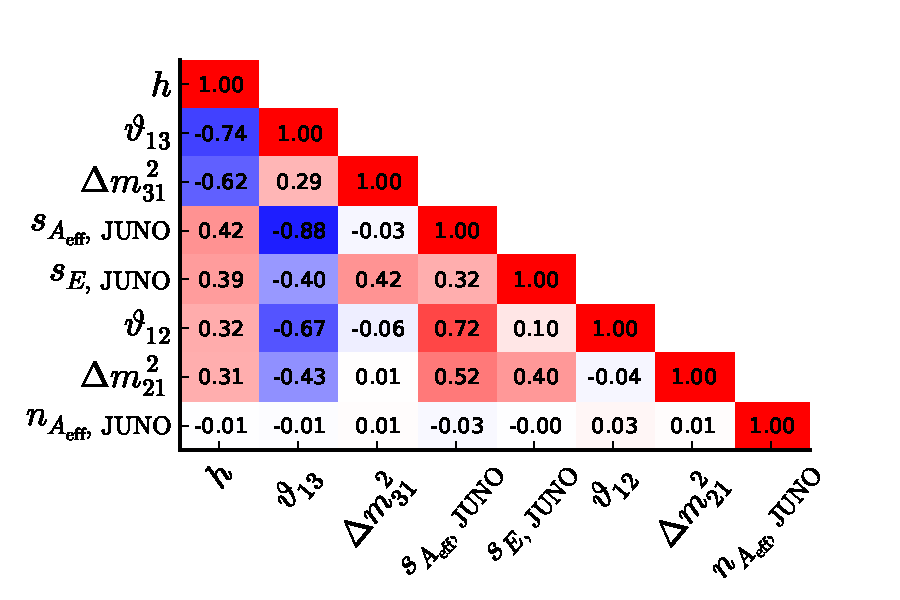
\includegraphics[width=0.7\linewidth]{CovMat_JUNO}
 \caption{Covariance matrix for JUNO, without external constraints on the
  oscillation parameters.}
 \label{fig:CovMat_JUNO}
\end{figure}

\noindent
Now that an observable has been constructed which is sufficiently linear as a
function of the parameters that JUNO will measure, the Fisher Matrix can be
applied.

The full error listing is given in Tab.~\ref{tab:JUNO_results}, where one can
read off a NMH sensitivity of $3.0\,\sigma$ for an event sample of
$N_\mathrm{tot} = 10^5$. Yet in contrast to the PINGU analysis, no priors have
been put on any of the oscillation parameters as the resulting significance is
to be compared to the one quoted by the JUNO collaboration themselves. In
\cite{JUNO2}, for a ``reactor-only analysis'', \ie no without external
knowledge, a confidence level of $\delchi^2 \approx 11$ is reported,
corresponding to a significance of $\mathcal{S} = \sqrt{\delchi^2} \approx
3.3\,\sigma$. This does not match up perfectly with the figure retrieved from
the modified \papa simulation, however the agreement is fairly good given that
the two calculations are completely independent in simulation and analysis
method, and in addition \papa was intended for a very different experiment.

Another claim from \cite{JUNO2} is that the NMH significance can be increased
to $\delchi^2 \approx 19\ \hat{=}\ \mathcal{S} \approx 4.4\,\sigma$ when using
a prior measurement of \dm{\mu\mu} with 1\,\% precision. This parameter can be
measured in \numu disappearance experiments, usually with a neutrino beam from
an accelerator travelling over a baseline of $\mathcal{O}$(100\,km). But since
\dm{\mu\mu} is a rather complex combination of all mixing parameters
\cite{Deltam_ee_mumu}, it is not possible to put the corresponding prior in the
base of mixing parameters chosen in this thesis.

One can, however, include priors on all mixing parameters according to a
current global fit \cite{Fogli} as it was done in the analysis for PINGU
(cf.\ Sec~\ref{sec:input_osc}). This increases the significance retrieved from
the Fisher Matrix to 4.6\,$\sigma$, a gain of 1.6\,$\sigma$ \wrt the value
without any priors. The full errors are listed in Tab.~\ref{tab:JUNO_priors}. In
JUNO's own analysis, only 1.1\,$\sigma$ are added by the inclusion of external
constraints, however there only one prior is put on an composite parameter,
which is a weaker statement than putting individual priors on four underlying
parameters.

The strongest impact on JUNO's expected sensitivity to the neutrino mass
hierarchy has the uncertainty of the mixing angle \thet{13}, as one can read
off from Tab.~\ref{tab:JUNO_results} and the covariance matrix, shown in
Fig.~\ref{fig:CovMat_JUNO}. Including the current knowledge of this parameter
alone enhances the significance to 4.4\,$\sigma$.

Next in size is the impact of \dm{31} on the mass hierarchy. For this parameter,
however, including the current knowledge as a prior does not significantly
improve the NMH measurement. The reason is that the current uncertainty on
\dm{31} is $8 \cdot 10^{-5}\,\mathrm{eV}^2$ \cite{Fogli}, while JUNO will
already provide a constraint of $1.7 \cdot 10^{-5}\,\mathrm{eV}^2$ by itself
(see Tab.~\ref{tab:JUNO_results}), \ie there is no other experiment that can
make a more precise measurement of \dm{31} than JUNO.

This sub-percent precision on the value of \dm{31} is stated by \cite{JUNO2},
too. A similar precision is claimed for \sinsq{\thet{12}} and \dm{21}. Looking
at Tab.~\ref{tab:JUNO_results}, that value can be reproduced for
\sinsq{\thet{12}}\footnote{} while for \dm{21} the relative uncertainty from
the Fisher matrix is on the order of 10\,\%. Yet in the given reference it
remains unclear whether the stated uncertainties include the prior on
\dm{\mu\mu}. After adding priors on all oscillation parameters but \dm{21}, the
Fisher matrix lists a precision of $\approx 3\,\%$ (see
Tab.~\ref{tab:JUNO_no_prior_dm21}).

\subsection{Joint Analysis of JUNO and PINGU}
\label{sec:JUNO_comb}